\title{Midterm 2 for Calculus-Based Physics-1: Mechanics (PHYS150-01)}
\author{Dr. Jordan Hanson - Whittier College Dept. of Physics and Astronomy}
\date{October 16th, 2017}
\documentclass[10pt]{article}
\usepackage[a4paper, total={18cm, 27cm}]{geometry}
\usepackage{outlines}
\usepackage[sfdefault]{FiraSans}
\usepackage{graphicx}

\begin{document}
\maketitle

\section{Vectors and Newton's Laws}
\begin{enumerate}
\item Let $\vec{F}_{\rm 1} = -\frac{3}{2}\hat{x} + 2\hat{y}$ N, and $\vec{F}_{\rm 2} = -2\hat{x} + \frac{3}{2}\hat{y}$ N.  a) Give the magnitude of each force.  b) What is the net force?  c) What is the angle between these two forces? \vspace{2.0 cm}
\item Imagine you are sitting in an airplane that has just lifted off with an acceleration vector 45 degrees with respect to horizontal.  Draw a free-body diagram corresponding to you, showing all forces acting on you.
\vspace{2.0 cm}
\item Imagine you are riding a skateboard down a hill.  Draw a free-body diagram corresponding to you, showing all forces acting on you.
\vspace{2.0 cm}
\end{enumerate}
\section{Newton's Laws, and Circular Motion}
\begin{figure}[ht]
\centering
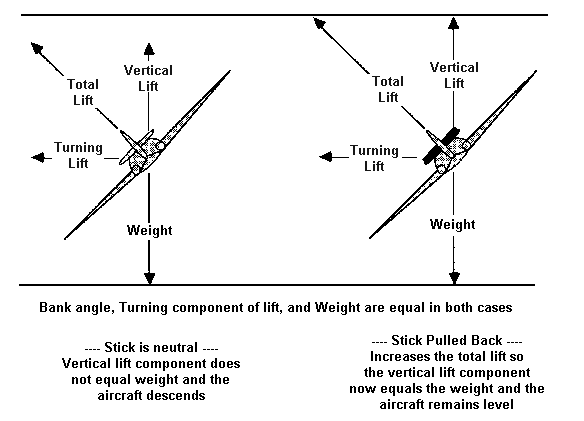
\includegraphics[width=0.2\textwidth,trim=10cm 4.84cm 0cm 0.6cm,clip=true]{bank.png}
\caption{\label{fig:bank} Let the weight be $\vec{w}$, and the total lift be $\vec{L}$, which may be be broken into two components: the turning force (equal to centripetal force $\vec{f}_{\rm C}$) and vertical lift (which balances weight).}
\end{figure}
\begin{enumerate}
\item When banking, the free-body diagram of a jet-fighter resembles Fig. \ref{fig:bank}.  To bank while maintaining altitude, the lift force $\vec{L}$ must \textit{both} balance the weight $\vec{w}$ and provide the centripetal force $\vec{f}_{\rm C}$.  Let the mass of the aircraft be $m$, the radius of the turn be $r$, and the angle between $\vec{L}$ and horizontal be $\theta$.
\begin{itemize}
\item Show that the angular velocity of the turn, $\omega$, is $\omega = \sqrt{\frac{L\cos\theta}{rm}}$ \vspace{3cm}
\item If $\omega$ is the angular velocity, then the \textit{period} is $T = 2\pi/\omega$.  This is the time required to fly in a complete circle.  Show that one-half period is $\frac{T}{2} = \pi\sqrt{\frac{r m}{L\cos\theta}}$.  This is the time required to turn.\vspace{3cm}
\item Let $L = 8\times 10^5$ N, $m = 2\times 10^4$ kg, $r = \frac{1}{2}$ km, and $\theta = 60$ degrees.  How long does it take the jet fighter to turn?\vspace{3cm}
\item What is the speed of the jet fighter?
\begin{itemize}
\item A: 10 m/s 
\item B: 20 m/s
\item C: 100 m/s
\item D: 120 m/s
\end{itemize}
\end{itemize} 
\end{enumerate}
\section{Frictional Forces}
\begin{enumerate}
\item There is a spill of a mystery toxic liquid on a shop floor, and no one wants to touch it.  Someone gets the bright idea that they can identify it by the coefficient of kinetic friction and a steel plate.  Draw a free body diagram corresponding to a steel plate sliding along the liquid/floor, with friction decelerating it.\vspace{2.5cm}
\item What is the coefficient of kinetic friction, $\mu_{\rm k}$, if a steel plate with an initial speed of 5 m/s comes to a stop after 2.5 seconds, assuming $g = 10$ m/s$^2$?  (Use the definition of acceleration $\Delta v/\Delta t = a$).
\begin{itemize}
\item 0.1
\item 0.2
\item 0.5
\item 1.2
\end{itemize}
\item Suppose they get a sample of the mystery liquid in a vile.  They assume the drag force is given by Stoke's Law, $F_{\rm D} = 6\pi r \eta v$, where $v$ is the velocity of a particle moving through they fluid, $r$ is the radius of the particle, and $\eta$ is the \textit{viscosity}.  They drop a bead with $r = 1$ mm and a mass of one gram into the fluid, and observe the bead sink with a constant (terminal) velocity of 1 m/s.  What is the viscosity of the fluid?  Units: kg/(m s).
\begin{itemize}
\item $5/(3\pi)$ kg/(m s)
\item $5/(30\pi)$ kg/(m s)
\item $10$ kg/(m s)
\item $5$ kg/(m s)
\end{itemize}
\end{enumerate}
\end{document}